% Yolymatics Tutorials — GCSE Distance-Time and Speed-Time Graphs Worksheet
% Build with: pdflatex gcse_distance_speed_time_graphs.tex

\documentclass[11pt,a4paper]{article}

% Core packages
\usepackage[margin=2cm]{geometry}
\usepackage[T1]{fontenc}
\usepackage[utf8]{inputenc}
\usepackage{lmodern}
\usepackage{amsmath, amssymb}
\usepackage{graphicx}
\usepackage{enumitem}
\usepackage{fancyhdr}
\usepackage{tcolorbox}
\usepackage{tikz}
\usepackage{pgfplots}
\usepackage{hyperref}

\pgfplotsset{compat=1.17}

% Professional brand colors
\definecolor{YolyPrimary}{HTML}{1E3A8A}   % deep professional blue
\definecolor{YolyAccent}{HTML}{F59E0B}    % warm amber
\definecolor{YolyDark}{HTML}{0F172A}      % slate dark
\definecolor{YolyLight}{HTML}{F8FAFC}     % very light gray

% Header and footer
\pagestyle{fancy}
\fancyhf{}
\fancyhead[L]{\textcolor{YolyPrimary}{\textbf{Yolymatics Tutorials}}}
\fancyhead[R]{\textcolor{YolyDark}{GCSE Mathematics}}
\fancyfoot[C]{\textcolor{YolyDark}{\thepage}}
\fancyfoot[R]{\textcolor{YolyAccent}{\href{mailto:yolymatics007@gmail.com}{yolymatics007@gmail.com}}}
\renewcommand{\headrulewidth}{2pt}
\renewcommand{\footrulewidth}{1pt}
\renewcommand{\headrule}{\hbox to\headwidth{\color{YolyAccent}\leaders\hrule height \headrulewidth\hfill}}
\renewcommand{\footrule}{\hbox to\headwidth{\color{YolyPrimary}\leaders\hrule height \footrulewidth\hfill}}

% Custom tcolorbox styles
\tcbuselibrary{skins,breakable}

\newtcolorbox{sectionbox}[1]{
  colback=YolyPrimary!5,
  colframe=YolyPrimary,
  fonttitle=\bfseries\large,
  title=#1,
  boxrule=2pt,
  arc=3mm,
  breakable
}

\newtcolorbox{problembox}[1]{
  colback=white,
  colframe=YolyAccent,
  fonttitle=\bfseries,
  title=#1,
  boxrule=1.5pt,
  arc=2mm,
  breakable
}

\newtcolorbox{tipbox}{
  colback=YolyAccent!10,
  colframe=YolyAccent,
  fonttitle=\bfseries,
  title=\textcolor{YolyDark}{Key Points},
  boxrule=1.5pt,
  arc=2mm
}

% Workspace command
\newcommand{\workspace}[1]{
  \vspace{#1}
}

\title{
  \textcolor{YolyPrimary}{\Huge\textbf{GCSE Mathematics}}\\
  \textcolor{YolyAccent}{\Large Distance-Time and Speed-Time Graphs}\\[0.5cm]
  \textcolor{YolyDark}{AQA Exam Preparation Worksheet}
}
\author{\textcolor{YolyPrimary}{\textbf{Yolymatics Tutorials}}}
\date{\textcolor{YolyDark}{\today}}

\begin{document}

\maketitle
\thispagestyle{fancy}

\vspace{0.5cm}
\begin{center}
  \begin{tcolorbox}[colback=YolyLight,colframe=YolyPrimary,width=0.8\textwidth,arc=3mm]
    \centering
    \textcolor{YolyDark}{\textbf{Student Name:} \underline{\hspace{6cm}}}\\[0.3cm]
    \textcolor{YolyDark}{\textbf{Date:} \underline{\hspace{6cm}}}
  \end{tcolorbox}
\end{center}

\vspace{0.5cm}
\begin{center}
  \textcolor{YolyDark}{\textit{Show all working clearly. Draw graphs using a ruler and pencil.}}
\end{center}

\newpage

% ===========================
% SECTION 1: DISTANCE-TIME GRAPHS - BASICS
% ===========================
\begin{sectionbox}{Part 1: Distance-Time Graphs — Understanding the Basics}
\vspace{0.3cm}

\begin{tipbox}
\textbf{Remember:}
\begin{itemize}
  \item The \textbf{gradient (slope)} of a distance-time graph = \textbf{speed}
  \item A \textbf{horizontal line} means stationary (not moving)
  \item A \textbf{steeper line} means faster speed
  \item Speed = $\frac{\text{distance}}{\text{time}}$
\end{itemize}
\end{tipbox}

\vspace{1cm}

\begin{problembox}{Problem 1: Reading distance-time graphs}
The graph below shows Sarah's journey to school.

\begin{center}
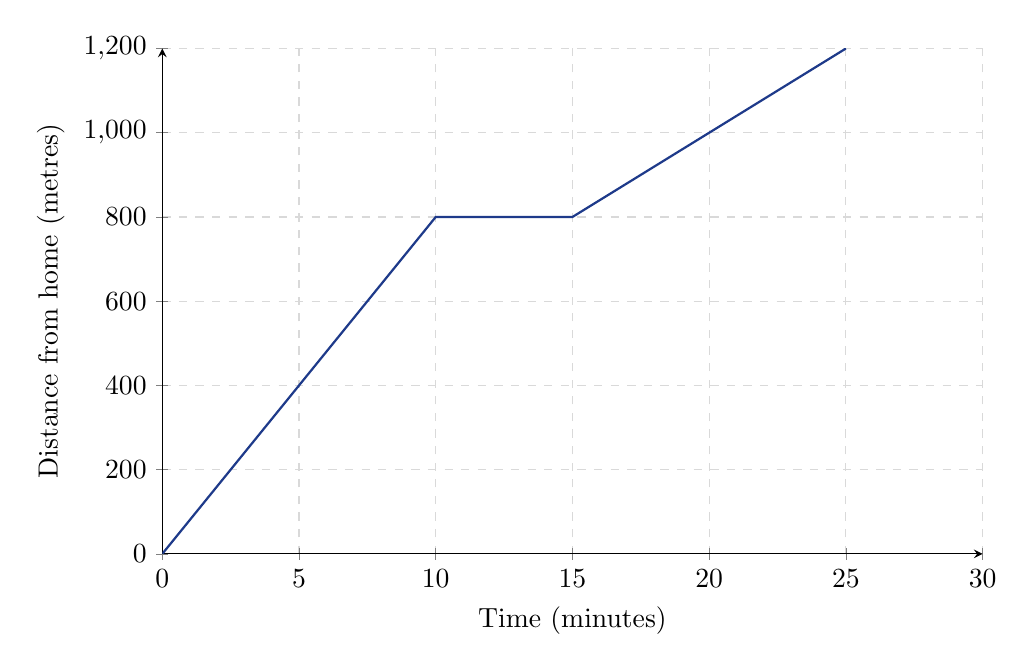
\begin{tikzpicture}
\begin{axis}[
    width=12cm, height=8cm,
    xlabel={Time (minutes)},
    ylabel={Distance from home (metres)},
    xmin=0, xmax=30,
    ymin=0, ymax=1200,
    xtick={0,5,10,15,20,25,30},
    ytick={0,200,400,600,800,1000,1200},
    grid=major,
    grid style={dashed,gray!30},
    axis lines=left,
    every axis plot/.append style={thick, YolyPrimary}
]
\addplot[YolyPrimary, thick] coordinates {
    (0,0) (10,800) (15,800) (25,1200)
};
\end{axis}
\end{tikzpicture}
\end{center}

\textbf{(a)} How far is Sarah's school from her home?

\workspace{2cm}

\textbf{(b)} How long did Sarah's whole journey take?

\workspace{2cm}

\textbf{(c)} For how long did Sarah stop during her journey?

\workspace{2cm}

\textbf{(d)} Calculate Sarah's speed during the first 10 minutes. Give your answer in metres per minute.

\workspace{3cm}

\textbf{(e)} Calculate Sarah's speed for the final part of her journey (from 15 to 25 minutes).

\workspace{3cm}

\textbf{(f)} During which part of the journey was Sarah travelling fastest? Explain your answer.

\workspace{2cm}
\end{problembox}

\end{sectionbox}

\newpage

\begin{sectionbox}{Part 1 continued: Distance-Time Graphs}

\begin{problembox}{Problem 2: Calculating speed from distance-time graphs}
Tom cycles from home to the library. The distance-time graph shows his journey.

\begin{center}
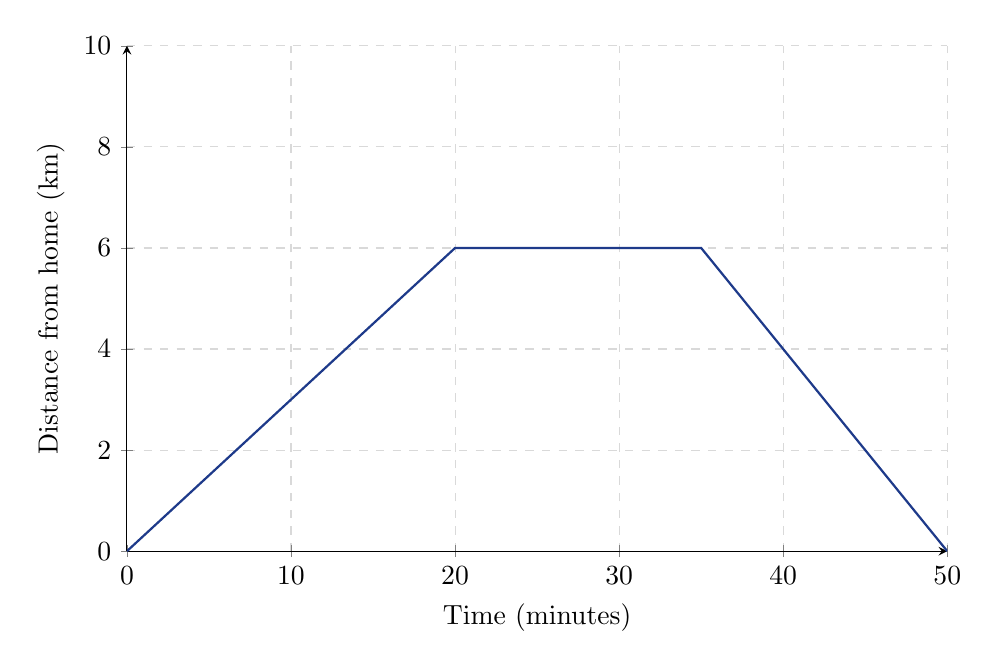
\begin{tikzpicture}
\begin{axis}[
    width=12cm, height=8cm,
    xlabel={Time (minutes)},
    ylabel={Distance from home (km)},
    xmin=0, xmax=50,
    ymin=0, ymax=10,
    xtick={0,10,20,30,40,50},
    ytick={0,2,4,6,8,10},
    grid=major,
    grid style={dashed,gray!30},
    axis lines=left,
    every axis plot/.append style={thick, YolyPrimary}
]
\addplot[YolyPrimary, thick] coordinates {
    (0,0) (20,6) (35,6) (50,0)
};
\end{axis}
\end{tikzpicture}
\end{center}

\textbf{(a)} How far is the library from Tom's home?

\workspace{2cm}

\textbf{(b)} Calculate Tom's speed on his way to the library. Give your answer in km/h.

\workspace{4cm}

\textbf{(c)} How long did Tom spend at the library?

\workspace{2cm}

\textbf{(d)} Calculate Tom's speed on his journey home. Give your answer in km/h.

\workspace{4cm}

\textbf{(e)} During which part of the journey was Tom travelling faster?

\workspace{2cm}
\end{problembox}

\end{sectionbox}

\newpage

\begin{sectionbox}{Part 1 continued: Drawing Distance-Time Graphs}

\begin{problembox}{Problem 3: Drawing a distance-time graph}
Emma walks to the shops. Here is a description of her journey:

\begin{itemize}
  \item She walks 600m in 10 minutes
  \item She stays at the shops for 15 minutes
  \item She walks back home, taking 12 minutes
\end{itemize}

\textbf{(a)} Draw a distance-time graph to represent Emma's journey on the axes below.

\begin{center}
\begin{tikzpicture}
\begin{axis}[
    width=14cm, height=10cm,
    xlabel={Time (minutes)},
    ylabel={Distance from home (metres)},
    xmin=0, xmax=40,
    ymin=0, ymax=800,
    xtick={0,5,10,15,20,25,30,35,40},
    ytick={0,100,200,300,400,500,600,700,800},
    grid=major,
    grid style={dashed,gray!30},
    axis lines=left
]
\end{axis}
\end{tikzpicture}
\end{center}

\textbf{(b)} Calculate Emma's speed on her way to the shops in metres per minute.

\workspace{3cm}

\textbf{(c)} Calculate Emma's speed on her way home in metres per minute.

\workspace{3cm}

\textbf{(d)} During which part of the journey was Emma walking faster?

\workspace{2cm}
\end{problembox}

\end{sectionbox}

\newpage

\begin{sectionbox}{Part 1 continued: Multi-Stage Journeys}

\begin{problembox}{Problem 4: Real-life journey}
James drives from Manchester to Birmingham, a distance of 150 km. Here is information about his journey:

\begin{itemize}
  \item He drives for 1 hour at a constant speed
  \item He stops at a service station for 30 minutes
  \item He continues driving for another hour at a constant speed
\end{itemize}

His journey takes 2.5 hours in total (including the stop).

\textbf{(a)} Draw a distance-time graph for James's journey on the axes below.

\begin{center}
\begin{tikzpicture}
\begin{axis}[
    width=14cm, height=10cm,
    xlabel={Time (hours)},
    ylabel={Distance from Manchester (km)},
    xmin=0, xmax=3,
    ymin=0, ymax=180,
    xtick={0,0.5,1,1.5,2,2.5,3},
    ytick={0,20,40,60,80,100,120,140,160,180},
    grid=major,
    grid style={dashed,gray!30},
    axis lines=left
]
\end{axis}
\end{tikzpicture}
\end{center}

\textbf{(b)} Calculate James's average speed for the whole journey (including the stop). Give your answer in km/h.

\workspace{3cm}

\textbf{(c)} How far had James travelled when he stopped at the service station?

\workspace{2cm}

\textbf{(d)} Calculate his speed for the first hour of driving.

\workspace{3cm}
\end{problembox}

\end{sectionbox}

\newpage

% ===========================
% SECTION 2: SPEED-TIME GRAPHS - BASICS
% ===========================
\begin{sectionbox}{Part 2: Speed-Time Graphs — Understanding the Basics}
\vspace{0.3cm}

\begin{tipbox}
\textbf{Remember:}
\begin{itemize}
  \item The \textbf{gradient (slope)} of a speed-time graph = \textbf{acceleration}
  \item A \textbf{horizontal line} means constant speed
  \item An \textbf{upward slope} means accelerating (speeding up)
  \item A \textbf{downward slope} means decelerating (slowing down)
  \item The \textbf{area under the graph} = \textbf{distance travelled}
  \item Acceleration = $\frac{\text{change in speed}}{\text{time}}$
\end{itemize}
\end{tipbox}

\vspace{1cm}

\begin{problembox}{Problem 5: Reading speed-time graphs}
The graph below shows a car's journey.

\begin{center}
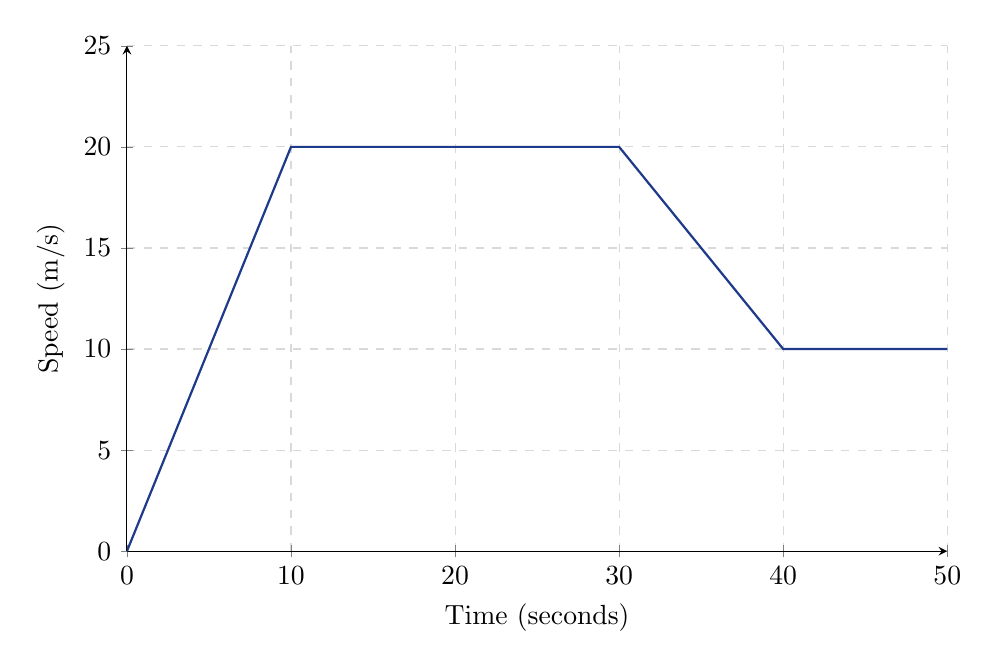
\begin{tikzpicture}
\begin{axis}[
    width=12cm, height=8cm,
    xlabel={Time (seconds)},
    ylabel={Speed (m/s)},
    xmin=0, xmax=50,
    ymin=0, ymax=25,
    xtick={0,10,20,30,40,50},
    ytick={0,5,10,15,20,25},
    grid=major,
    grid style={dashed,gray!30},
    axis lines=left,
    every axis plot/.append style={thick, YolyPrimary}
]
\addplot[YolyPrimary, thick] coordinates {
    (0,0) (10,20) (30,20) (40,10) (50,10)
};
\end{axis}
\end{tikzpicture}
\end{center}

\textbf{(a)} What was the car's maximum speed?

\workspace{2cm}

\textbf{(b)} For how long did the car travel at constant speed?

\workspace{2cm}

\textbf{(c)} Calculate the car's acceleration during the first 10 seconds. Give your answer in m/s².

\workspace{3cm}

\textbf{(d)} Calculate the deceleration between 30 and 40 seconds. Give your answer in m/s².

\workspace{3cm}

\textbf{(e)} Describe what happened to the car between 40 and 50 seconds.

\workspace{2cm}
\end{problembox}

\end{sectionbox}

\newpage

\begin{sectionbox}{Part 2 continued: Calculating Distance from Speed-Time Graphs}

\begin{problembox}{Problem 6: Finding distance travelled}
A train's journey is shown on the speed-time graph below.

\begin{center}
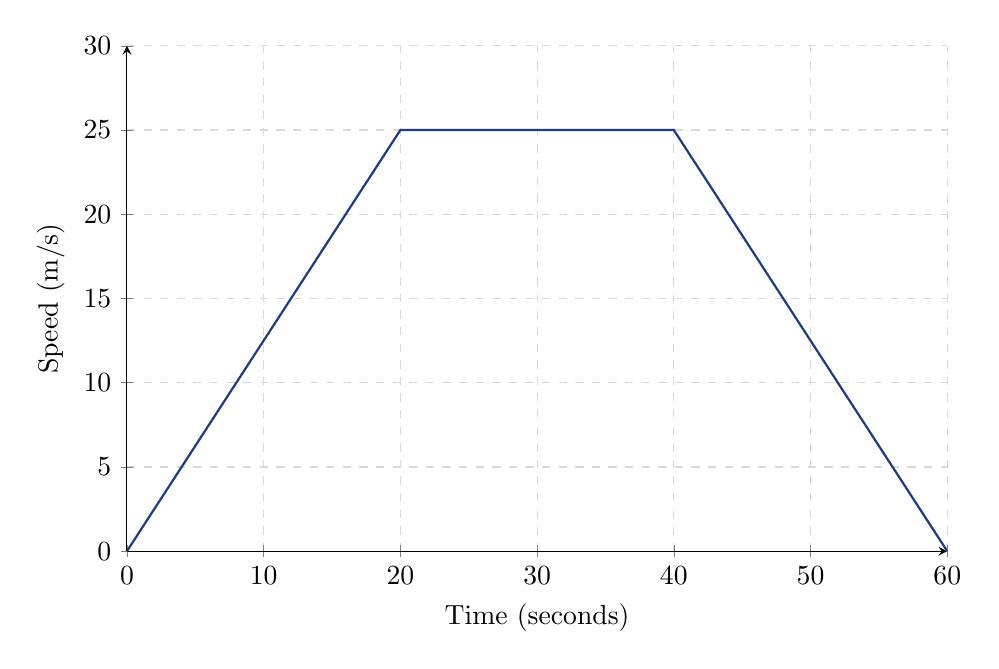
\begin{tikzpicture}
\begin{axis}[
    width=12cm, height=8cm,
    xlabel={Time (seconds)},
    ylabel={Speed (m/s)},
    xmin=0, xmax=60,
    ymin=0, ymax=30,
    xtick={0,10,20,30,40,50,60},
    ytick={0,5,10,15,20,25,30},
    grid=major,
    grid style={dashed,gray!30},
    axis lines=left,
    every axis plot/.append style={thick, YolyPrimary}
]
\addplot[YolyPrimary, thick] coordinates {
    (0,0) (20,25) (40,25) (60,0)
};
\end{axis}
\end{tikzpicture}
\end{center}

\textbf{(a)} Calculate the train's acceleration during the first 20 seconds.

\workspace{3cm}

\textbf{(b)} Calculate the distance travelled by the train during the first 20 seconds.
\textit{(Hint: The area is a triangle. Area of triangle = $\frac{1}{2} \times \text{base} \times \text{height}$)}

\workspace{4cm}

\textbf{(c)} Calculate the distance travelled between 20 and 40 seconds.

\workspace{3cm}

\textbf{(d)} Calculate the distance travelled during the final 20 seconds.

\workspace{4cm}

\textbf{(e)} What is the total distance travelled by the train?

\workspace{2cm}
\end{problembox}

\end{sectionbox}

\newpage

\begin{sectionbox}{Part 2 continued: Drawing Speed-Time Graphs}

\begin{problembox}{Problem 7: Drawing a speed-time graph}
A cyclist's journey is described below:

\begin{itemize}
  \item She accelerates from rest to 8 m/s in 4 seconds
  \item She travels at 8 m/s for 10 seconds
  \item She decelerates uniformly to rest in 6 seconds
\end{itemize}

\textbf{(a)} Draw a speed-time graph for the cyclist's journey on the axes below.

\begin{center}
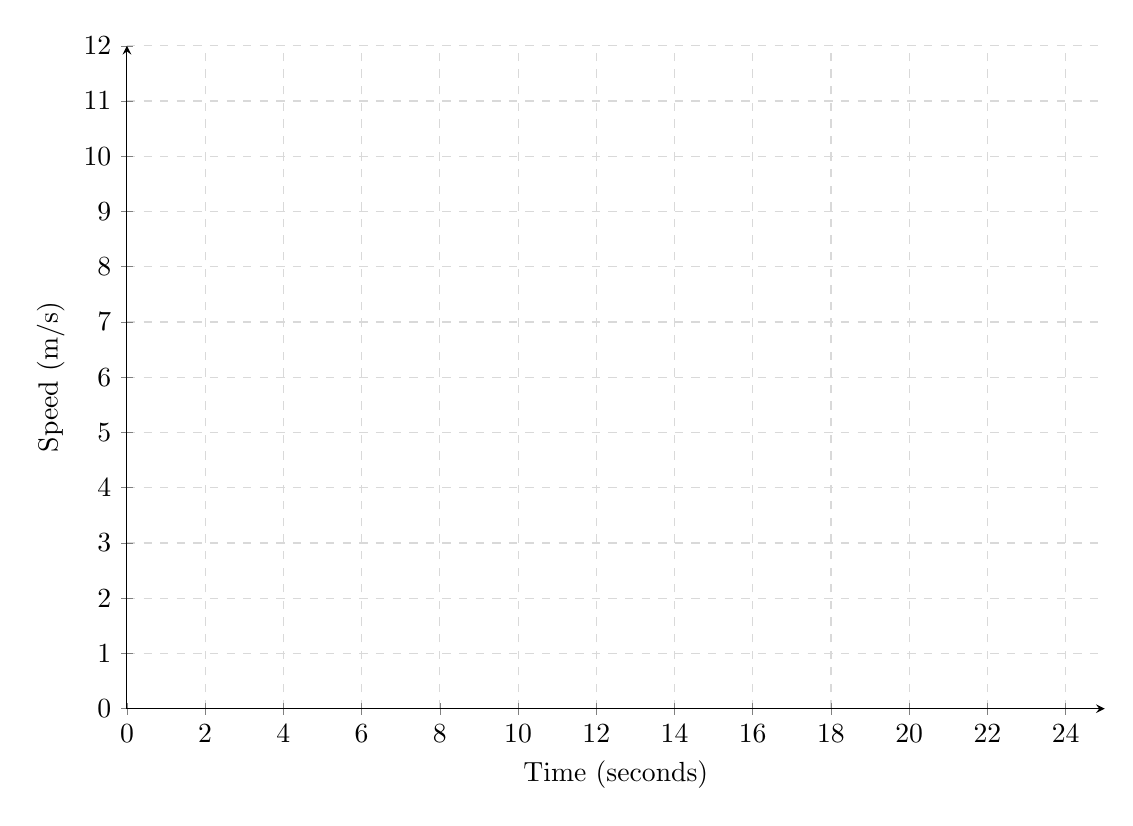
\begin{tikzpicture}
\begin{axis}[
    width=14cm, height=10cm,
    xlabel={Time (seconds)},
    ylabel={Speed (m/s)},
    xmin=0, xmax=25,
    ymin=0, ymax=12,
    xtick={0,2,4,6,8,10,12,14,16,18,20,22,24},
    ytick={0,1,2,3,4,5,6,7,8,9,10,11,12},
    grid=major,
    grid style={dashed,gray!30},
    axis lines=left
]
\end{axis}
\end{tikzpicture}
\end{center}

\textbf{(b)} Calculate the cyclist's acceleration during the first 4 seconds.

\workspace{3cm}

\textbf{(c)} Calculate the total distance travelled by the cyclist.

\workspace{5cm}

\textbf{(d)} Calculate the cyclist's average speed for the whole journey.

\workspace{3cm}
\end{problembox}

\end{sectionbox}

\newpage

\begin{sectionbox}{Part 2 continued: Complex Speed-Time Graphs}

\begin{problembox}{Problem 8: Real-life scenario — Bus journey}
A bus journey is shown on the speed-time graph below.

\begin{center}
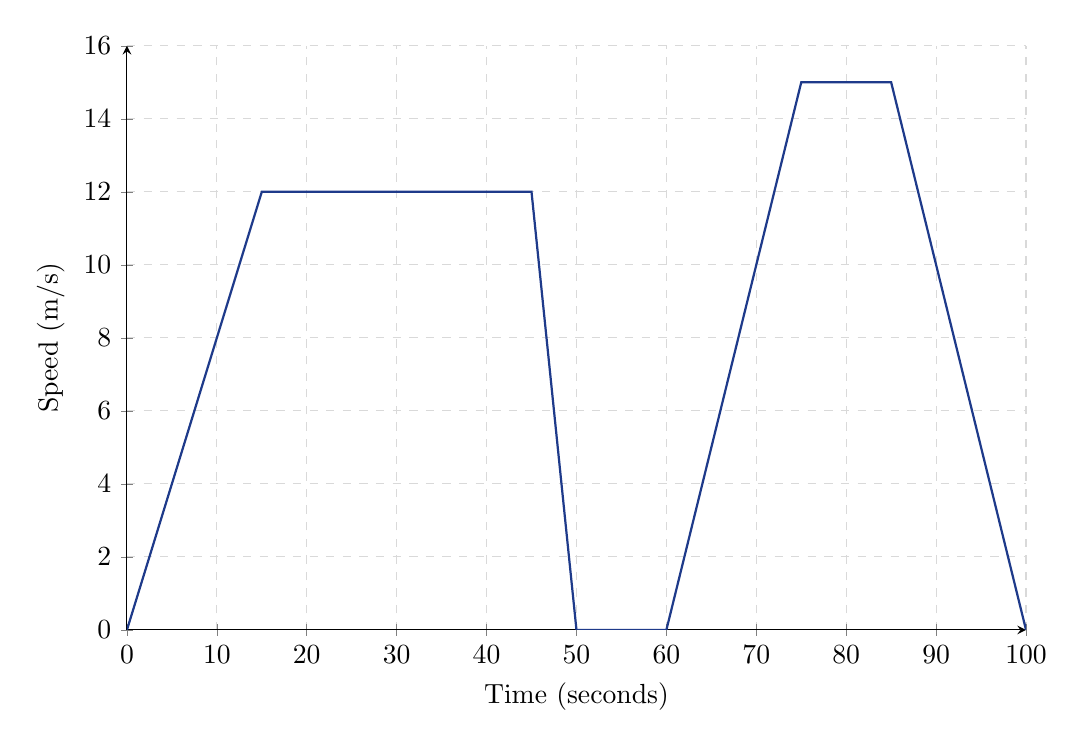
\begin{tikzpicture}
\begin{axis}[
    width=13cm, height=9cm,
    xlabel={Time (seconds)},
    ylabel={Speed (m/s)},
    xmin=0, xmax=100,
    ymin=0, ymax=16,
    xtick={0,10,20,30,40,50,60,70,80,90,100},
    ytick={0,2,4,6,8,10,12,14,16},
    grid=major,
    grid style={dashed,gray!30},
    axis lines=left,
    every axis plot/.append style={thick, YolyPrimary}
]
\addplot[YolyPrimary, thick] coordinates {
    (0,0) (15,12) (45,12) (50,0) (60,0) (75,15) (85,15) (100,0)
};
\end{axis}
\end{tikzpicture}
\end{center}

\textbf{(a)} What was the maximum speed of the bus?

\workspace{2cm}

\textbf{(b)} For how long was the bus stationary (stopped)?

\workspace{2cm}

\textbf{(c)} Calculate the acceleration during the first 15 seconds.

\workspace{3cm}

\textbf{(d)} Calculate the total distance travelled by the bus. 
\textit{(Hint: Split the graph into shapes — triangles, rectangles, and trapeziums)}

\workspace{8cm}

\textbf{(e)} Calculate the average speed for the whole journey.

\workspace{3cm}
\end{problembox}

\end{sectionbox}

\newpage

% ===========================
% SECTION 3: COMPARING GRAPHS
% ===========================
\begin{sectionbox}{Part 3: Comparing Distance-Time and Speed-Time Graphs}

\begin{problembox}{Problem 9: Two runners}
Ali and Ben run a 400m race. The distance-time graph shows their race.

\begin{center}
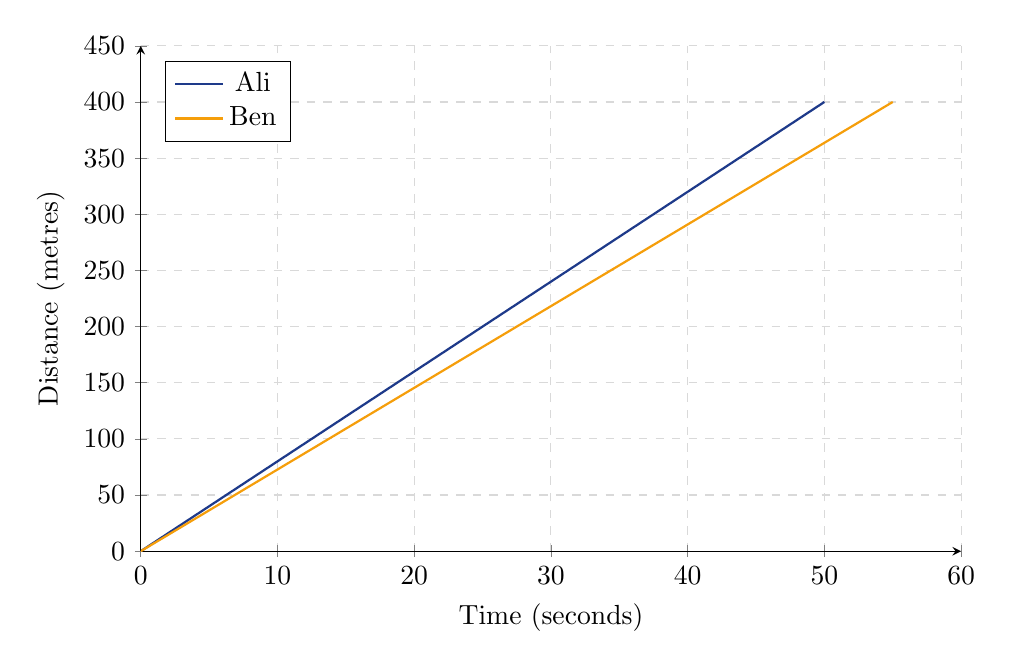
\begin{tikzpicture}
\begin{axis}[
    width=12cm, height=8cm,
    xlabel={Time (seconds)},
    ylabel={Distance (metres)},
    xmin=0, xmax=60,
    ymin=0, ymax=450,
    xtick={0,10,20,30,40,50,60},
    ytick={0,50,100,150,200,250,300,350,400,450},
    grid=major,
    grid style={dashed,gray!30},
    axis lines=left,
    legend pos=north west
]
\addplot[YolyPrimary, thick] coordinates {
    (0,0) (50,400)
};
\addlegendentry{Ali}

\addplot[YolyAccent, thick] coordinates {
    (0,0) (55,400)
};
\addlegendentry{Ben}
\end{axis}
\end{tikzpicture}
\end{center}

\textbf{(a)} Who won the race?

\workspace{1.5cm}

\textbf{(b)} What was the time difference between the two runners?

\workspace{2cm}

\textbf{(c)} Calculate Ali's speed in metres per second.

\workspace{3cm}

\textbf{(d)} Calculate Ben's speed in metres per second.

\workspace{3cm}

\textbf{(e)} Who was running faster? By how much?

\workspace{2cm}
\end{problembox}

\end{sectionbox}

\newpage

\begin{sectionbox}{Part 3 continued: Interpreting Multiple Journeys}

\begin{problembox}{Problem 10: Car overtaking}
Two cars, Car A and Car B, are travelling along a motorway. The speed-time graph shows their motion.

\begin{center}
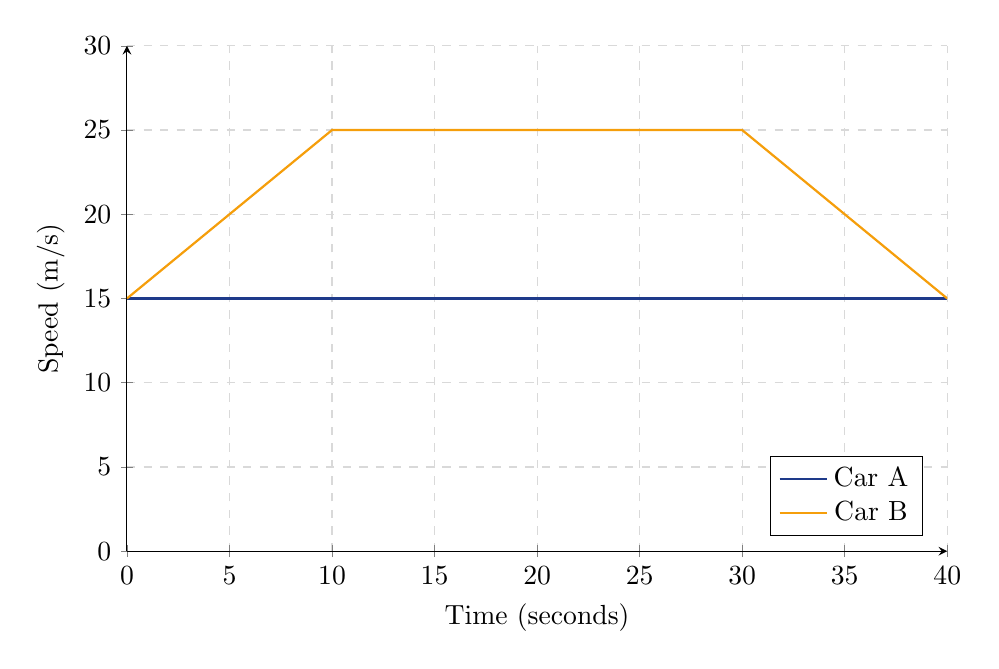
\begin{tikzpicture}
\begin{axis}[
    width=12cm, height=8cm,
    xlabel={Time (seconds)},
    ylabel={Speed (m/s)},
    xmin=0, xmax=40,
    ymin=0, ymax=30,
    xtick={0,5,10,15,20,25,30,35,40},
    ytick={0,5,10,15,20,25,30},
    grid=major,
    grid style={dashed,gray!30},
    axis lines=left,
    legend pos=south east
]
\addplot[YolyPrimary, thick] coordinates {
    (0,15) (40,15)
};
\addlegendentry{Car A}

\addplot[YolyAccent, thick] coordinates {
    (0,15) (10,25) (30,25) (40,15)
};
\addlegendentry{Car B}
\end{axis}
\end{tikzpicture}
\end{center}

\textbf{(a)} What was Car A's speed throughout the journey?

\workspace{2cm}

\textbf{(b)} Calculate Car B's acceleration during the first 10 seconds.

\workspace{3cm}

\textbf{(c)} Calculate the distance travelled by Car A during the 40 seconds.

\workspace{3cm}

\textbf{(d)} Calculate the distance travelled by Car B during the 40 seconds.

\workspace{5cm}

\textbf{(e)} Which car travelled further? By how much?

\workspace{2cm}
\end{problembox}

\end{sectionbox}

\newpage

% ===========================
% SECTION 4: EXAM-STYLE QUESTIONS
% ===========================
\begin{sectionbox}{Part 4: Exam-Style Questions}

\begin{problembox}{Problem 11: Multi-part exam question (Higher Tier)}
A delivery van travels from a warehouse to a shop and back. The speed-time graph shows the van's journey.

\begin{center}
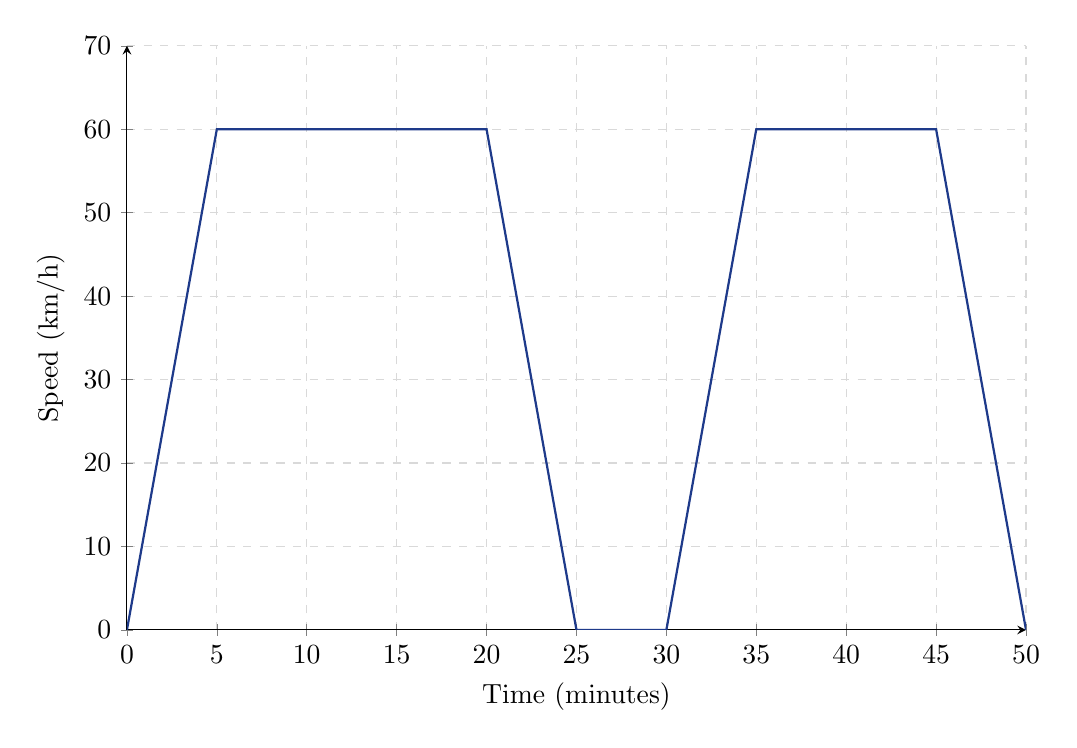
\begin{tikzpicture}
\begin{axis}[
    width=13cm, height=9cm,
    xlabel={Time (minutes)},
    ylabel={Speed (km/h)},
    xmin=0, xmax=50,
    ymin=0, ymax=70,
    xtick={0,5,10,15,20,25,30,35,40,45,50},
    ytick={0,10,20,30,40,50,60,70},
    grid=major,
    grid style={dashed,gray!30},
    axis lines=left,
    every axis plot/.append style={thick, YolyPrimary}
]
\addplot[YolyPrimary, thick] coordinates {
    (0,0) (5,60) (20,60) (25,0) (30,0) (35,60) (45,60) (50,0)
};
\end{axis}
\end{tikzpicture}
\end{center}

\textbf{(a)} Calculate the van's acceleration during the first 5 minutes. Give your answer in km/h per minute.

\workspace{3cm}

\textbf{(b)} Calculate the distance travelled by the van during the first 20 minutes.
\textit{(Remember: Area under graph = distance. You may need to convert units)}

\workspace{5cm}

\textbf{(c)} For how long was the van stationary during the whole journey?

\workspace{2cm}

\textbf{(d)} Calculate the total distance travelled during the whole 50-minute journey.

\workspace{6cm}

\textbf{(e)} The shop is 18 km from the warehouse. Show that the van travelled further on the return journey than on the outward journey.

\workspace{4cm}
\end{problembox}

\end{sectionbox}

\newpage

\begin{sectionbox}{Part 4 continued: Challenge Questions}

\begin{problembox}{Problem 12: Creating your own graph}
Lucy walks from home to the park, stays at the park, then walks back home. 
The distance from her home to the park is 1.5 km. Here is information about her journey:

\begin{itemize}
  \item She walks to the park at 5 km/h
  \item She stays at the park for 30 minutes
  \item She walks home at 4 km/h
\end{itemize}

\textbf{(a)} Calculate how long it takes Lucy to walk to the park. Give your answer in minutes.

\workspace{3cm}

\textbf{(b)} Calculate how long it takes Lucy to walk home. Give your answer in minutes.

\workspace{3cm}

\textbf{(c)} Draw a distance-time graph for Lucy's complete journey on the axes below.

\begin{center}
\begin{tikzpicture}
\begin{axis}[
    width=14cm, height=10cm,
    xlabel={Time (minutes)},
    ylabel={Distance from home (km)},
    xmin=0, xmax=80,
    ymin=0, ymax=2,
    xtick={0,10,20,30,40,50,60,70,80},
    ytick={0,0.25,0.5,0.75,1,1.25,1.5,1.75,2},
    grid=major,
    grid style={dashed,gray!30},
    axis lines=left
]
\end{axis}
\end{tikzpicture}
\end{center}

\textbf{(d)} Calculate Lucy's average speed for the whole journey (including the time at the park).

\workspace{3cm}
\end{problembox}

\end{sectionbox}

\newpage

\begin{sectionbox}{Part 4 continued: Word Problems}

\begin{problembox}{Problem 13: Train journey (Exam-style)}
A train travels between two stations, A and B, which are 30 km apart.

The train:
\begin{itemize}
  \item Accelerates uniformly from rest to 25 m/s in 100 seconds
  \item Travels at 25 m/s for 15 minutes
  \item Decelerates uniformly to rest in 80 seconds
\end{itemize}

\textbf{(a)} Draw a speed-time graph for the train's journey. Use the axes below.
\textit{(Remember: 15 minutes = 900 seconds)}

\begin{center}
\begin{tikzpicture}
\begin{axis}[
    width=14cm, height=9cm,
    xlabel={Time (seconds)},
    ylabel={Speed (m/s)},
    xmin=0, xmax=1200,
    ymin=0, ymax=30,
    xtick={0,100,200,300,400,500,600,700,800,900,1000,1100,1200},
    ytick={0,5,10,15,20,25,30},
    grid=major,
    grid style={dashed,gray!30},
    axis lines=left
]
\end{axis}
\end{tikzpicture}
\end{center}

\textbf{(b)} Calculate the train's acceleration.

\workspace{3cm}

\textbf{(c)} Calculate the total distance travelled by the train. Give your answer in metres.

\workspace{6cm}

\textbf{(d)} Convert your answer to part (c) to kilometres.

\workspace{2cm}

\textbf{(e)} Does the train complete its journey between stations A and B? Explain your answer.

\workspace{3cm}
\end{problembox}

\end{sectionbox}

\newpage

% ===========================
% SECTION 5: MIXED PRACTICE
% ===========================
\begin{sectionbox}{Part 5: Mixed Practice and Challenge Questions}

\begin{problembox}{Problem 14: Cyclist and walker}
A cyclist and a walker both leave town A at the same time, heading for town B which is 20 km away.

\begin{itemize}
  \item The cyclist travels at a constant speed of 16 km/h
  \item The walker travels at a constant speed of 4 km/h
\end{itemize}

\textbf{(a)} On the same axes below, draw distance-time graphs for both the cyclist and the walker.

\begin{center}
\begin{tikzpicture}
\begin{axis}[
    width=14cm, height=10cm,
    xlabel={Time (hours)},
    ylabel={Distance from town A (km)},
    xmin=0, xmax=6,
    ymin=0, ymax=22,
    xtick={0,0.5,1,1.5,2,2.5,3,3.5,4,4.5,5,5.5,6},
    ytick={0,2,4,6,8,10,12,14,16,18,20,22},
    grid=major,
    grid style={dashed,gray!30},
    axis lines=left
]
\end{axis}
\end{tikzpicture}
\end{center}

\textbf{(b)} How long does it take the cyclist to reach town B?

\workspace{3cm}

\textbf{(c)} How far apart are the cyclist and walker after 30 minutes?

\workspace{4cm}

\textbf{(d)} The cyclist rests at town B for 45 minutes, then cycles back towards town A at 16 km/h.
Add this to your graph above. At what time do the cyclist and walker meet?

\workspace{4cm}
\end{problembox}

\end{sectionbox}

\newpage

\begin{sectionbox}{Part 5 continued: Challenge Problem}

\begin{problembox}{Problem 15: Ultimate challenge (Higher Tier)}
A car journey consists of three stages:

\textbf{Stage 1:} The car accelerates from rest to 30 m/s in 15 seconds

\textbf{Stage 2:} The car travels at 30 m/s for 2 minutes

\textbf{Stage 3:} The car decelerates to 10 m/s in 10 seconds, then continues at 10 m/s for 45 seconds

\textbf{(a)} Draw a speed-time graph for the complete journey on the axes below.

\begin{center}
\begin{tikzpicture}
\begin{axis}[
    width=14cm, height=9cm,
    xlabel={Time (seconds)},
    ylabel={Speed (m/s)},
    xmin=0, xmax=200,
    ymin=0, ymax=35,
    xtick={0,20,40,60,80,100,120,140,160,180,200},
    ytick={0,5,10,15,20,25,30,35},
    grid=major,
    grid style={dashed,gray!30},
    axis lines=left
]
\end{axis}
\end{tikzpicture}
\end{center}

\textbf{(b)} Calculate the total time for the journey.

\workspace{2cm}

\textbf{(c)} Calculate the acceleration in Stage 1.

\workspace{3cm}

\textbf{(d)} Calculate the deceleration in Stage 3.

\workspace{3cm}

\textbf{(e)} Calculate the total distance travelled during the entire journey.

\workspace{7cm}

\textbf{(f)} Calculate the average speed for the whole journey in m/s.

\workspace{3cm}
\end{problembox}

\end{sectionbox}

\newpage

% ===========================
% SUMMARY AND FORMULAS
% ===========================
\begin{center}
  \begin{tcolorbox}[colback=YolyAccent!10,colframe=YolyAccent,width=0.9\textwidth,arc=4mm,boxrule=2pt]
    \begin{center}
      {\Large\textcolor{YolyPrimary}{\textbf{Summary — Key Formulas and Tips}}}
    \end{center}
    
    \vspace{0.5cm}
    
    \textbf{\textcolor{YolyPrimary}{Distance-Time Graphs:}}
    \begin{itemize}
      \item Gradient = Speed
      \item Horizontal line = Stationary
      \item Steeper line = Faster speed
      \item Speed = $\frac{\text{Distance}}{\text{Time}}$
    \end{itemize}
    
    \vspace{0.5cm}
    
    \textbf{\textcolor{YolyPrimary}{Speed-Time Graphs:}}
    \begin{itemize}
      \item Gradient = Acceleration
      \item Horizontal line = Constant speed
      \item Area under graph = Distance travelled
      \item Acceleration = $\frac{\text{Change in speed}}{\text{Time}}$
    \end{itemize}
    
    \vspace{0.5cm}
    
    \textbf{\textcolor{YolyPrimary}{Important Conversions:}}
    \begin{itemize}
      \item 1 km = 1000 m
      \item 1 hour = 60 minutes = 3600 seconds
      \item To convert km/h to m/s: divide by 3.6
      \item To convert m/s to km/h: multiply by 3.6
    \end{itemize}
    
    \vspace{0.5cm}
    
    \textbf{\textcolor{YolyPrimary}{Area Formulas:}}
    \begin{itemize}
      \item Rectangle: length × width
      \item Triangle: $\frac{1}{2} \times \text{base} \times \text{height}$
      \item Trapezium: $\frac{1}{2} \times (\text{sum of parallel sides}) \times \text{height}$
    \end{itemize}
  \end{tcolorbox}
\end{center}

\vspace{1cm}

\begin{center}
  \begin{tcolorbox}[colback=YolyPrimary!10,colframe=YolyPrimary,width=0.9\textwidth,arc=4mm,boxrule=2pt]
    \begin{center}
      {\Large\textcolor{YolyPrimary}{\textbf{Excellent Work!}}}\\[0.5cm]
      \textcolor{YolyDark}{You have completed comprehensive practice on distance-time}\\
      \textcolor{YolyDark}{and speed-time graphs for your GCSE exam preparation.}\\[0.8cm]
      {\large\textcolor{YolyAccent}{\textbf{Yolymatics Tutorials}}}\\
      \textcolor{YolyDark}{\href{mailto:yolymatics007@gmail.com}{yolymatics007@gmail.com}}
    \end{center}
  \end{tcolorbox}
\end{center}

\vfill

\begin{center}
  \textcolor{YolyDark}{\textit{Good luck with your AQA GCSE Mathematics exam!}}
\end{center}

\end{document}
